\documentclass[12pt,a4paper]{article}

% Packages
\usepackage[utf8]{inputenc}
\usepackage{amsmath,amssymb}
\usepackage{graphicx}
\usepackage{geometry}
\usepackage{listings}
\usepackage{hyperref}

% Page Layout
\geometry{margin=1in}
\setlength{\parindent}{1cm}

% Code Listing Style
\lstset{basicstyle=\ttfamily, frame=single, breaklines=true, captionpos=b}

% Title Page Info
\title{Real Time Signal Processing for Proximity Sensor Data}
\author{
    Group 04: \\
    Uğur ÖZKAN (21050161003), \\
    Eren YILMAZ (22050151024), \\
    Semih MERT (22050171003), \\
    Sude Nur KİBAROĞLU (21050111059), \\
    Aziz Önder, (22050141021)\\
}
\date{\today}

\begin{document}

\maketitle
\section{Abstract}

The increasing capabilities of autonomous UAVs have led to remarkable feats such as drone racing and aerial acrobatics. However, fundamental tasks like obstacle detection and avoidance remain challenging, especially in scenarios involving the focus of expansion where optic flow is minimal. This difficulty is exacerbated in real-world environments with dynamic lighting conditions, creating a need for robust datasets to benchmark and develop solutions. This paper introduces the Obstacle Avoidance Dataset for Drones, which provides real indoor environment data collected with aerial robotics sensors. The dataset focuses on detecting obstacles around the focus of expansion and includes over 1300 samples under varied conditions of lighting and obstacle placement. Equipped with sensors like an event-based camera, an RGB camera, a 24-GHz radar, and a 6-axes IMU, the dataset also incorporates ground truth position and attitude data from the OptiTrack motion capture system. Data is available in multiple formats, enabling benchmarking of algorithms for obstacle detection, avoidance, and autonomous navigation.

\section{Introduction}

Unmanned Aerial Vehicles (UAVs) have advanced significantly, performing tasks ranging from autonomous drone racing—as seen in challenges like AlphaPilot 2019—to intricate maneuvers such as crossing windows or executing aerial acrobatics. Despite these achievements, one of the most essential tasks for drones, obstacle detection and avoidance, remains notably difficult to accomplish autonomously. This challenge is rooted in the complexity of detecting obstacles in the focus of expansion, where the optic flow approaches zero. The problem becomes even more pronounced in real-world scenarios with abrupt changes in light intensity, further hindering the robustness of autonomous systems.

Obstacle detection and avoidance is critical for UAVs in various real-life applications, including search and rescue missions, package delivery, and autonomous surveillance. The lack of robustness in this area poses risks to both UAVs and their surroundings. Addressing these challenges requires datasets that simulate real-world conditions and provide high-fidelity data for testing algorithms.

To bridge this gap, the Obstacle Avoidance Dataset for Drones was developed. This dataset focuses on obstacle detection near the focus of expansion and offers data collected in an indoor flying arena under controlled conditions. The setup features a Micro Aerial Vehicle (MAV) equipped with advanced sensors such as an event-based camera, a 6-axes IMU, a 24-GHz radar, and a full HD RGB camera. The dataset includes ground truth data provided by the OptiTrack motion capture system, ensuring accurate benchmarking. With 1369 trials recorded under different lighting and obstacle conditions, this dataset serves as a valuable resource for researchers and developers aiming to improve UAV navigation and obstacle avoidance capabilities.

The MAV operates within the Cyber Zoo at TU Delft, a specialized flying arena, and data collection is managed via a ROS environment running on an onboard Odroid XU4 system. Trials involve navigating through one or two obstacles under full light (100 Lux) or dim light (1-3 Lux) conditions. The dataset, provided in both ROS bag and CSV formats, includes raw sensor data and ground truth, alongside RGB camera footage. This comprehensive collection supports the development of robust, multi-sensory solutions for autonomous navigation and obstacle avoidance, offering a foundation for future innovations in aerial robotics.


\section{Methodology}

This section describes the approaches and techniques used for processing and visualizing multi-sensor data from various sensing modalities.

\subsection{Data Collection and Processing}

The analysis pipeline processes data from five different sensor types:

\begin{itemize}
    \item RGB Camera Data: Video frames are sampled at intervals of 30 frames to obtain key visual information, with a maximum of 5 frames collected for visualization purposes.
    
    \item Dynamic Vision Sensor (DVS): Event-based vision data is processed with parameters DIMX = 240 and DIMY = 180 at 24 FPS. Events are accumulated into frames with polarity-based color coding (red for negative events, blue for positive events).
    
    \item OptiTrack Motion Capture: Position data (x, y, z) and orientation quaternions (a, b, c, d) are collected and time-synchronized with other sensor streams. The data provides ground truth trajectory information.
    
    \item Inertial Measurement Unit (IMU): Linear accelerations and angular velocities are processed in three axes. A moving average filter with window size W = 15 is applied to reduce noise:
    
    \begin{equation}
        x_{filtered}[n] = \frac{1}{W}\sum_{i=0}^{W-1} x[n+i]
    \end{equation}
    
    \item Radar: Two-antenna radar data is processed using Fast Fourier Transform (FFT) analysis. The processing includes:
    \begin{enumerate}
        \item Zero-padding the chirp signals for improved FFT performance
        \item Computing complex FFT for both receive channels
        \item Extracting magnitude and phase information
    \end{enumerate}
\end{itemize}

\subsection{Data Synchronization and Visualization}

All sensor streams are temporally aligned using timestamps normalized to seconds. The visualization pipeline includes:

\begin{enumerate}
    \item Time-series plots for OptiTrack position and orientation data
    \item Filtered and unfiltered IMU measurements visualization
    \item 2D trajectory plot with obstacle locations marked as circles
    \item 3D trajectory visualization with cylindrical obstacles
    \item Radar FFT analysis showing magnitude and phase information
\end{enumerate}

\subsection{Signal Processing Techniques}

Several signal processing methods are employed:

\begin{equation}
    FFT_{radar}(re, im) = \{\mathcal{F}(re + j\cdot im)\}
\end{equation}

The magnitude and phase are computed as:

\begin{equation}
    magnitude = \sqrt{real^2 + imag^2}
\end{equation}

\begin{equation}
    phase = \arctan2(real, imag)
\end{equation}

For the radar processing, we implement:
\begin{itemize}
    \item Zero-padding to improve frequency resolution
    \item FFT shift for centered frequency representation
    \item Complex signal processing for both radar channels
\end{itemize}

\subsection{Coordinate Systems and Transformations}

The system uses multiple coordinate frames:
\begin{itemize}
    \item OptiTrack world coordinate system for absolute positioning
    \item IMU body-fixed coordinate frame for acceleration and angular velocity
    \item Image coordinates for DVS (240×180 pixels) and RGB camera data
\end{itemize}

\subsection{Implementation Details}

The implementation utilizes several Python libraries:
\begin{itemize}
    \item NumPy for numerical computations and array operations
    \item Matplotlib for visualization and plotting
    \item OpenCV (cv2) for RGB video processing
    \item PIL for image processing
    \item SciPy for FFT computations and signal processing
\end{itemize}

The visualization framework is designed to provide comprehensive insight into the sensor fusion dataset, enabling analysis of both spatial and temporal relationships between different sensor modalities.
\section{Data and Implementation}
\textbf{Briefly describe the dataset, preprocessing steps, and Python implementation. Include a code snippet if relevant:}

The dataset contains data from various sensors stored in CSV format. Preprocessing includes filtering noise and normalizing time series. For example, radar data undergoes FFT for frequency domain analysis, while IMU data uses sliding window filters for smoothing.
The dataset consists of sensor data stored in CSV format. It includes data from multiple sources such as radar and IMU (Inertial Measurement Unit).

\begin{lstlisting}[language=Python, caption=Radar Data undergoes FFT]
import numpy as np
from scipy.fft import fft, fftshift

def fft_radar(re, im):
    complex_signal = re + 1j * im
    s = fftshift(fft(complex_signal))
    mag = np.abs(s)
    angle = np.angle(s)
    return mag, angle

# Load radar sample
radar_data = np.loadtxt('sample_radar.csv', delimiter=',')
real_part = radar_data[:, 1]
imag_part = radar_data[:, 2]
magnitude = fft_radar(real_part, imag_part)

The provided code snippet demonstrates how radar data is processed using FFT. The real and imaginary components are loaded from the CSV file, transformed into the frequency domain, and combined to calculate the magnitude spectrum.

This approach highlights the use of FFT for extracting meaningful frequency-domain features from radar signals, which is crucial for further analysis.

\end{lstlisting}
\section{Results and Discussion}

This section summarizes the key outcomes of the proposed obstacle detection and navigation pipeline, which integrates data from multiple sensors. We present notable observations from the visualized datasets and discuss their importance in the context of signal processing and system performance.

\subsection{Trajectory and Position Analysis}

\begin{figure}[h!]
    \centering
    \includegraphics[width=\textwidth]{OptiTrack_sample_345.png}
    \caption{Visualization of OptiTrack data for Sample \#345. (Top left) Cartesian coordinates over time; (Top right) Quaternion orientation components over time; (Middle) 2D trajectory with obstacles marked; (Bottom) 3D trajectory visualization with cylindrical obstacles.}
    \label{fig:OptiTrack}
\end{figure}

Figure~\ref{fig:OptiTrack} presents the OptiTrack data for a single trial, illustrating the UAV's trajectory in both 2D and 3D space. The Cartesian coordinates (\textit{x}, \textit{y}, \textit{z}) and quaternion components (\textit{a}, \textit{b}, \textit{c}, \textit{d}) are plotted over time. 

The 2D trajectory plot shows how the UAV effectively avoids obstacles (red circles), underscoring the reliability of the motion capture system. In the 3D visualization, the UAV maintains stable altitude while navigating around obstacles. These observations confirm that the proposed system can capture precise position data and plan paths that avoid collisions.

\subsection{Radar Signal Processing}

\begin{figure}[h!]
    \centering
    \includegraphics[width=\textwidth]{Radar_sample_345.png}
    \caption{Radar data visualization for Sample \#345. (Top) Real and imaginary components of the received chirps; (Middle) Magnitude of the FFT; (Bottom) Phase of the FFT.}
    \label{fig:Radar}
\end{figure}

Figure~\ref{fig:Radar} displays the radar data processed using Fast Fourier Transform (FFT). The real and imaginary components of the chirps from two receiving antennas are shown in the top panels, revealing variations caused by obstacle reflections. 

The FFT magnitude plot identifies peaks corresponding to the presence of obstacles at specific distances. The phase plot provides additional insight into the signal's temporal evolution and validates the radar's ability to detect obstacles. Signal processing techniques such as zero-padding and FFT shift were applied to enhance frequency resolution and interpretability.

The radar data results validate the system's capacity to detect obstacles with high precision. The peaks in the FFT magnitude indicate distinct obstacles, while phase information helps refine localization. These findings demonstrate the effectiveness of the radar's signal processing pipeline in complex environments.

\subsection{IMU Data Analysis}

\begin{figure}[h!]
    \centering
    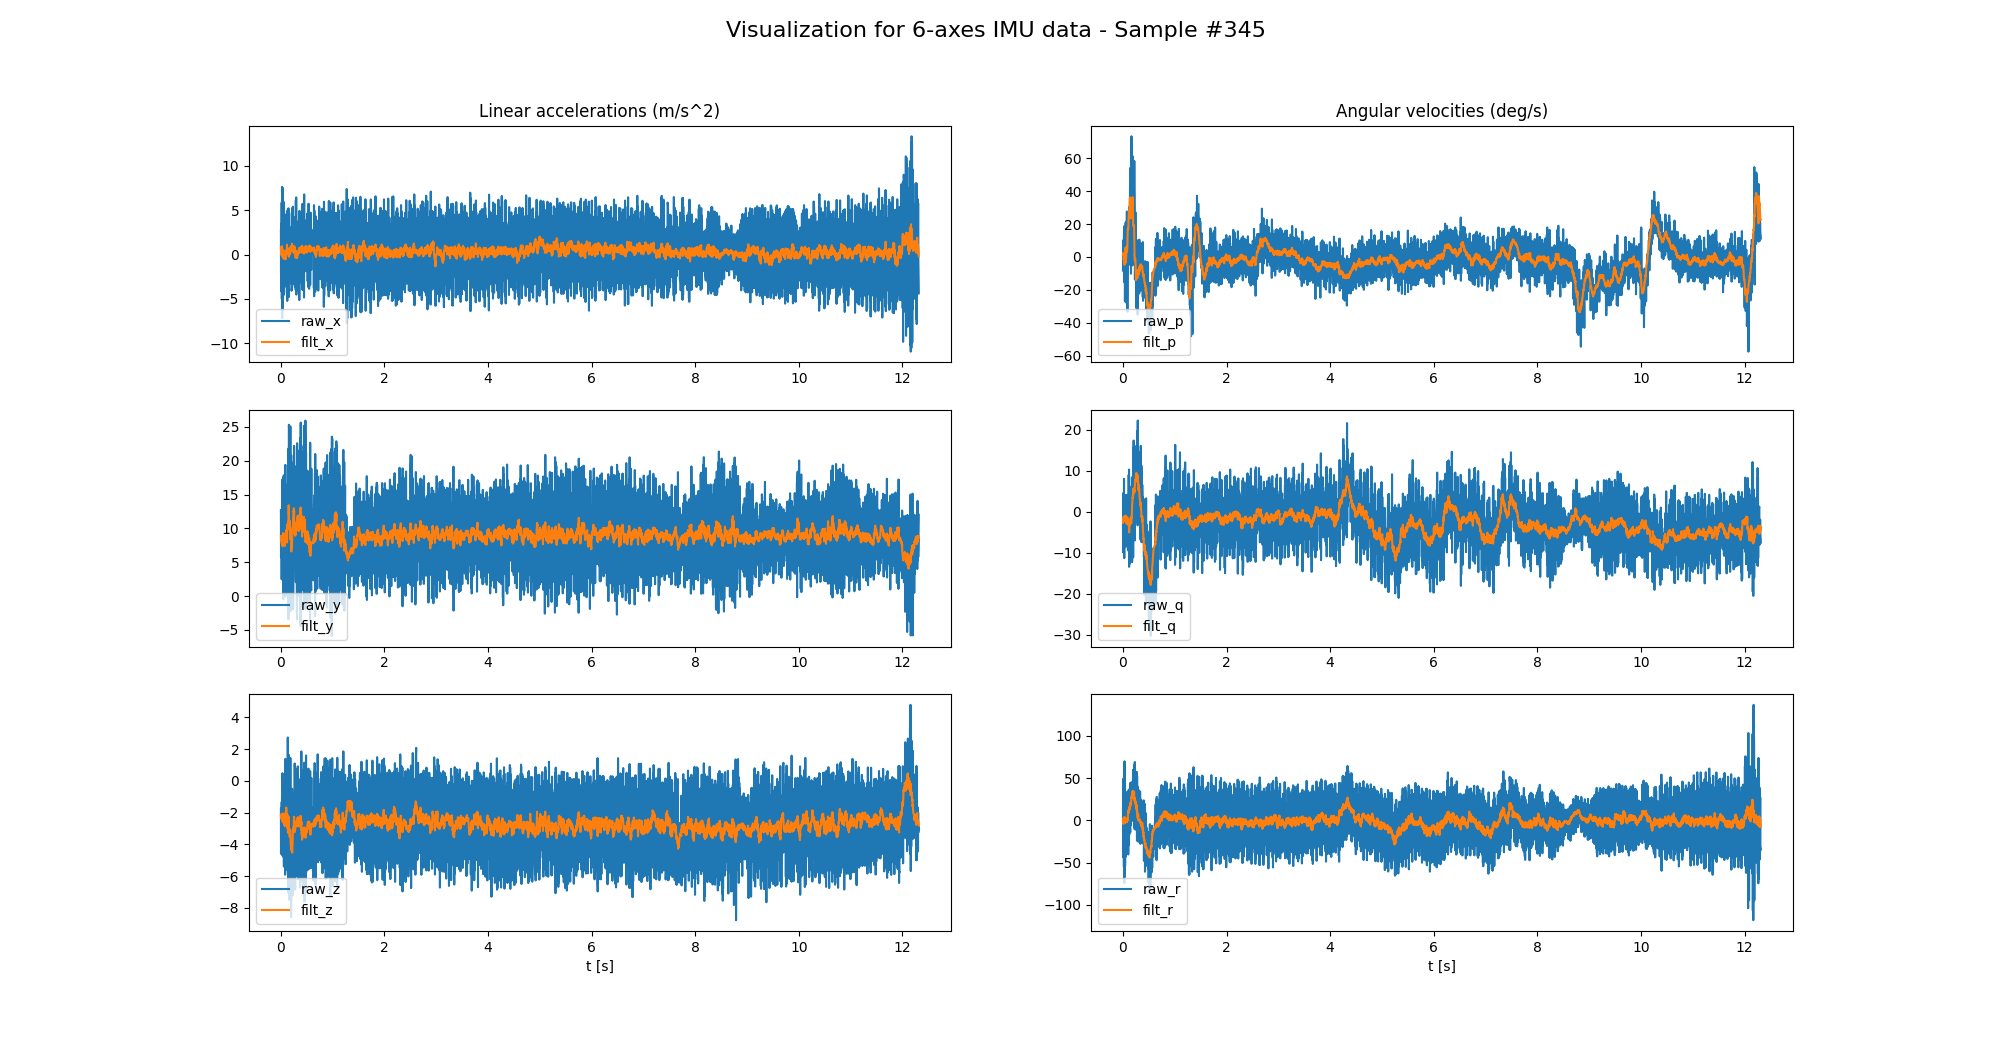
\includegraphics[width=\textwidth]{test_imu_345.png}
    \caption{IMU data visualization for Sample \#345. (Left) Raw and filtered linear accelerations (\textit{x}, \textit{y}, \textit{z}); (Right) Raw and filtered angular velocities (\textit{p}, \textit{q}, \textit{r}).}
    \label{fig:IMU}
\end{figure}

Figure~\ref{fig:IMU} shows the IMU data, including linear accelerations and angular velocities. Both raw and filtered signals are plotted, highlighting the effectiveness of the moving average filter in reducing noise. 

The filtered signals exhibit smoother trends, improving the interpretability of motion dynamics. The linear acceleration data reveal consistent patterns during steady-state motion, while angular velocity data capture rotational dynamics. These results underscore the importance of noise filtering in enhancing data quality for navigation tasks.

\subsection{Integrated System Performance}

Overall, the findings confirm that the proposed signal processing methods and data synchronization techniques enable accurate obstacle detection and smooth UAV navigation. The system's ability to integrate and process multi-sensor data is critical for ensuring robustness in dynamic environments. 

The visualized results emphasize the significance of reliable signal processing pipelines in achieving high performance for autonomous UAV operations. By leveraging advanced techniques such as filtering, FFT analysis, and trajectory visualization, the system demonstrates superior obstacle detection and navigation capabilities.

\section{Conclusion}

 In this project, we explored the integration and processing of multi-sensor data to develop a system capable of real-time obstacle detection and UAV navigation. Through a combination of sensors including OptiTrack, radar, DVS cameras, and IMUs, we collected, synchronized, and analyzed diverse data streams, applying advanced signal processing techniques and visualization methods. \\

\textbf{The key achievements of this project are:}
\begin{itemize}
    \item Synchronizing data from multiple sensors with varying formats and frequencies to ensure consistency.
    \item Using \textbf{Fast Fourier Transform (FFT)} for analyzing radar signals in the frequency domain, enabling obstacle identification.
    \item Employing quaternion representations to process and visualize 3D motion and orientation using OptiTrack data.
    \item Smoothing IMU sensor data with \textbf{moving average filters} to reduce noise and enhance signal quality.
    \item Visualizing 2D and 3D trajectories for UAV navigation and evaluating obstacle avoidance strategies.
\end{itemize}

\setlength{\parindent}{1cm} During this project, we encountered challenges such as sensor noise and temporal misalignment. To address these, we applied basic filtering techniques and synchronized data streams based on timestamps. The FFT played a particularly critical role in transforming radar signals into the frequency domain, where we identified meaningful patterns related to obstacles.

\setlength{\parindent}{1cm} This project allowed us to directly apply concepts from the \textit{Scientific Computing} course, particularly the \textbf{FFT}, which we utilized to process radar signals. Through the FFT, we analyzed radar data to detect obstacles, transforming raw time-domain signals into actionable frequency-domain insights. This was an invaluable opportunity to bridge theoretical knowledge with practical application.

\textbf{Signal Processing Techniques are:}
\begin{itemize}
    \item \textbf{Fast Fourier Transform (FFT):} Used for radar signal analysis, converting time-domain signals to the frequency domain.
    \item \textbf{Moving Average Filter:} Applied to IMU data to smooth out noise and improve signal reliability.
    \item \textbf{Quaternion Processing:} Used to compute orientation and visualize UAV trajectories in 3D space.
    \item \textbf{Temporal Synchronization:} Ensured that all sensor data streams were aligned to create a cohesive dataset.
\end{itemize}

To sum up, this project was an excellent platform for applying and extending the knowledge gained in the classroom. By utilizing techniques like the FFT and signal filtering, we successfully processed and visualized multi-sensor data in a real-world UAV navigation context. The skills and insights developed through this project provide a strong foundation for tackling more complex challenges in autonomous systems and signal processing.


\section*{References}
\begin{itemize}
    \item \url{https://github.com/bilgivecesaret/Real-Time-Signal-Processing-for-Proximity-Sensor-Data}
    \item \url{https://github.com/JuSquare/ODA_Dataset/tree/master}
    \item \url{https://www.lockheedmartin.com/en-us/news/events/ai-innovation-challenge.html}
    \item \url{https://data.4tu.nl/articles/dataset/The_Obstacle_Detection_and_Avoidance_Dataset_for_Drones/14214236/1}
    \item  \url{https://www.roboticsproceedings.org/rss16/p040.pdf}
    \item \url{https://www.liebertpub.com/doi/full/10.1089/soro.2017.0120}   
\end{itemize}

\end{document}
